\section{The exponential polynomial closed form}
\label{section:solspace}
We begin by discussing the exponential polynomial closed form, a perspective that is routinely leveraged to study the behaviour of Linear Recurrence Sequences. Simple LRS (no repeated characteristic roots) have the closed form
\begin{equation}
\label{eq:exppoly}
u_n = \sum_j w_j \rho_j^n + \sum_j (z_j \gamma_j^n + \bar{z_j}\bar{\gamma_j}^n)
\end{equation}
where each $\rho_j, \gamma_j, \bar{\gamma_j}$ are distinct roots of the characteristic polynomial. By straightforward arithmetic on the above expression, we can see that if $(u_n)_{n\in \naturals}, (v_n)_{n\in \naturals}$ are simple LRS with sets of characteristic roots $U$ and $V$ respectively, then
\begin{itemize}
\item $r_n = u_n + v_n$ is a simple LRS, whose set of roots is $U \cup V$.
\item $r_n = u_n \cdot v_n$ is a simple LRS, whose set of roots is $\{\gamma_1\gamma_2: \gamma_1 \in U, \gamma_2 \in V\}$.
\end{itemize}

In general, one can encode a linear recurrence $\mathbf{a}$ as a $\kappa \times \kappa$ companion matrix $\mathbf{A}$, and interpret the initialisation $\mathbf{c}$ as a vector. Then, $u_n$ is given by the first coordinate of $\mathbf{A}^n\mathbf{c}$, i.e.
\begin{equation}
\label{eq:companion}
\begin{bmatrix}
u_n \\
u_{n+1} \\
\vdots \\
u_{n+\kappa-1}
\end{bmatrix} 
= 
\begin{bmatrix}
0 & 1 & 0 & \dots & 0 \\
0 & 0 & 1 & \dots & 0 \\
\vdots & \vdots & \vdots & \dots & \vdots \\
a_0 & a_1 & a_2 & \dots & a_{\kappa-1}
\end{bmatrix}^n
\begin{bmatrix}
u_0 \\
u_{1} \\
\vdots \\
u_{\kappa-1}
\end{bmatrix}.
\end{equation}
Let $\mathbf{e_1}^T$ denote the row vector $\begin{bmatrix}1 & 0 & \dots & 0\end{bmatrix}$. We can thus write $u_n = \mathbf{e_1}^T\mathbf{A}^n\mathbf{c}$. It is now a standard fact that LRS have the following \textbf{real exponential polynomial} closed form 
\begin{equation}
\label{eq:realexppoly}
u_n = \left(\sum_{j=1}^{k_1}\sum_{\ell = 0}^{m_j-1} z_{j\ell}\rho_j^n n^\ell\right) + \left(\sum_{j=k_1 + 1}^{k_2} \sum_{\ell = 0}^{m_j-1} (x_{j\ell} \cos n\theta_j + y_{j\ell}\sin n\theta_j)\rho_j^n n^\ell\right)
\end{equation}
where $\rho_j$ (alternately, $\rho_j e^{i\theta_j}$) are roots of the characteristic polynomial defined by $\mathbf{a}$, each with multiplicity $m_j$. The coefficients $z_{j\ell}, x_{j\ell}, y_{j\ell}$ each depend linearly on $\mathbf{c}$. $u_n$ can thus be equivalently expressed as the inner (dot) product $\seq{\mathbf{p}, \mathbf{q_n}}$ where $\{\mathbf{q_n}\}_{n\in \naturals}$ is the sequence of vectors of terms that occur in the exponential polynomial expression, and $\mathbf{p}$ is the vector of corresponding coefficients. The choice of $\{\mathbf{q_n}\}_{n\in \naturals}$ can differ in ``phase'': one can replace $\cos n\theta, \sin n\theta$ by $\cos (n\theta-\varphi), \sin(n\theta-\varphi)$ for some choice of $\varphi$, and adjust the coefficients in $\mathbf{p}$ accordingly.

Roots such that $|\rho_j|$ is the largest are called \textbf{dominant}. The growth rate of a term in the above expression is governed by $\rho_j^n n^\ell$. Terms with the fastest growth are called \textbf{dominant terms}, and they drive the asymptotic behaviour of the LRS. A standard, intuitive prerequisite for Ultimate Positivity is that the leading terms in the exponential polynomial expression must include one that is real and strictly positive, otherwise their dominant contribution oscillates between positive and negative. It is formalised by applying \cite[Lemma 4]{Braverman06} to the dominant terms in expression \ref{eq:realexppoly} and arguing that the contribution from the remaining terms vanishes asymptotically. 
\begin{proposition}
\label{prop:folklore}
If the characteristic polynomial has no real dominant root of maximum multiplicity, then in any full-dimensional neighbourhood of initialisations, there exists an initialisation, such that the sequence has infinitely many positive terms, and infinitely many negative terms.
\end{proposition}

\textbf{Henceforth, we assume that the characteristic polynomial has a real positive dominant root of maximum multiplicity, for otherwise the answer to Ultimate Positivity is trivially NO.} 

We define $\seq{\mathbf{p}, \mathbf{q_n}}_{dom}$ to be the normalised contribution of the dominant terms in the exponential polynomial solution. That is, if the dominant growth rate is $\rho^n n^\ell$, we pick terms with that growth rate, and divide their contribution by $\rho^n n^\ell$. For example, if
$
u_n = p_1 2^n + p_2 2^n\cos (n\theta -\varphi) + p_3 2^n \sin (n\theta-\varphi) + p_4
$
then $$\seq{\mathbf{p}, \mathbf{q_n}}_{dom} = p_1  + p_2 \cos (n\theta-\varphi) + p_3 \sin (n\theta-\varphi).$$
We define
$
\mu(\mathbf{c}) = \liminf_{n \in \naturals} \seq{\mathbf{p}, \mathbf{q_n}}_{dom}.
$
Note that $\mu$ is an intrinsic property of the initialisation $\mathbf{c}$ and the sequence it generates, and hence is invariant under the choice of ``phase shift'' $\varphi$ while defining $\{\mathbf{q_n}\}_{n\in \naturals}$.

\section{Robust Positivity Problems}
\label{section:problems}

In this paper, we shall focus on defining and tackling Robust Positivity problems. Our input consists of a linear recurrence relation $\mathbf{a}$, an initialisation $\mathbf{c}$, and a positive definite matrix $\mathbf{S}$ that is used to define a neighbourhood around $\mathbf{c}$. \textbf{All input is real algebraic.}

\begin{problem}[$\mathbf{S}$-Robust Positivity]
\label{prob:rrobpos}
Decide whether for all $\mathbf{c'}$ such that $(\mathbf{c'} - \mathbf{c})^T\mathbf{S}(\mathbf{c'} - \mathbf{c}) \le 1$, the LRS $(\mathbf{a}, \mathbf{c'})$ is positive.
\end{problem}

\begin{problem}[$\mathbf{S}$-Robust Uniform Ultimate Positivity]
\label{prob:rrobuniultpos}
Decide whether there exists an $N$ such that for all $\mathbf{c'}$ with $(\mathbf{c'} - \mathbf{c})^T\mathbf{S}(\mathbf{c'} - \mathbf{c}) \le 1$, the LRS $(\mathbf{a}, \mathbf{c'})$ is positive from the $N^{th}$ term onwards.
\end{problem}

We can switch the order in which $N$ and $\mathbf{c'}$ are quantified, and query a weaker notion of Robust Ultimate Positivity:
\begin{problem}[$\mathbf{S}$-Robust Non-uniform Ultimate Positivity]
\label{prob:rrobnonuniultpos}
Decide whether for all $\mathbf{c'}$ with $(\mathbf{c'} - \mathbf{c})^T\mathbf{S}(\mathbf{c'} - \mathbf{c}) \le 1$ , there exists an $N$ such that the LRS $(\mathbf{a}, \mathbf{c'})$ is positive from the $N^{th}$ term onwards.
\end{problem}

The attentive reader might have already noticed that we depart from convention and specify neighbourhoods as \textit{closed} balls. Although \cite{originalarxiv} does not solve the problems we consider in this paper, it makes crucial observations about the geometry: for Problems \ref{prob:rrobpos} and \ref{prob:rrobuniultpos}, there is no difference between open and closed balls. On the other hand, Problem \ref{prob:rrobnonuniultpos} becomes considerably easier with open balls, and its decidability in this case is tackled in \cite{originalarxiv} itself. 

\subsection{Uniform Variants: The foundation}
\label{section:uniformfoundation}
In general, an arbitrary point $\mathbf{c'}$ is expressed as $\mathbf{c} + \mathbf{d}$, where $\mathbf{d} \in \mathcal{P}$, a full-dimensional neighbourhood symmetric about the origin. Observe equation \ref{eq:companion}. The $n^{th}$ term of the LRS is non-negative throughout the neighbourhood if and only if for all $d \in \mathcal{P}$,
$
\mathbf{e_1}^T \mathbf{A}^n (\mathbf{c + d}) \ge 0.
$
We can use the symmetry of $\mathcal{P}$ about the origin to rewrite the above as
\begin{equation}
\label{eq:illustrate}
\mathbf{e_1}^T \mathbf{A}^n \mathbf{c}\ge \max_{\mathbf{d} \in \mathcal{P}} \mathbf{e_1}^T\mathbf{A}^n\mathbf{d} \ge 0.
\end{equation}
As a simple illustration, assume that the neighbourhood is defined by a polytope rather than a positive definite matrix. This situation arises, for instance, when the metric is based on the $\ell^1$- or $\ell^\infty$-norm, as opposed to the $\ell^2$-norm.  In this simple example, $\mathcal{P}$ is a polytope, hence $\mathbf{e_1}^T\mathbf{A}^n\mathbf{d}$ is maximised at one of the finitely many corners $\{\mathbf{d_1}, \dots, \mathbf{d_k}\}$. Thus, Robust (Uniform Ultimate) Positivity is decided by using the state of the art \cite{joeljames3} to check the (Ultimate) Positivity of each of the LRS $(\mathbf{a}, \mathbf{c+d_i})$. The geometry of our setting is not simple enough to allow such a straightforward approach.
\textbf{The overview of our approach to Problems \ref{prob:rrobpos} and \ref{prob:rrobuniultpos} is as follows.}
\begin{enumerate}
\item Decide (constructively for Problem \ref{prob:rrobpos}) whether there exists an $N_1$ such that $\mathbf{e_1}^T \mathbf{A}^n \mathbf{c} \ge 0$ for all $n > N_1$. If $N_1$ is explicitly required, the state of the art is able to tackle LRS of order $\le 5$ \cite{joeljames3} and Simple LRS of order $\le 9$ \cite{ouaknine2014positivity}. In the non-constructive case, it can further handle all simple LRS \cite{ouaknine2014ultimate}.
\item Use linear-algebraic arguments to define a real algebraic LRS $(v_n)_{n=0}^\infty$, such that $v_n \ge 0$ if and only if $|\mathbf{e_1}^T \mathbf{A}^n \mathbf{c}|\ge \max_{\mathbf{d} \in \mathcal{P}} \mathbf{e_1}^T\mathbf{A}^n\mathbf{d}$.
\item Decide (constructively for Problem \ref{prob:rrobpos}) whether there exists $N_2$ such that $v_n \ge 0$ for all $n > N_2$. Positivity throughout the neighbourhood is thus guaranteed beyond step $N = \max(N_1, N_2)$. If either $N_1$ or $N_2$ does not exist, then Robust Ultimate Positivity, and hence Robust Positivity, does not hold.
\item \textbf{Only for Problem \ref{prob:rrobpos}:} Explicitly check inequality \ref{eq:illustrate} for $n \le N$.
\end{enumerate}

Our novelty lies in Step 2 and identifying when Step 3 can be implemented. We now discuss how we perform Steps 2 and 4 when $\mathcal{P} = \mathcal{B}_\mathbf{S}$, a neighbourhood of vectors $\mathbf{d}$ such that $\mathbf{d}^T\mathbf{S}\mathbf{d} \le 1$. The defining parameter $\mathbf{S}$ is a real algebraic positive definite matrix. We note that since $\mathbf{S}$ is positive definite, it can be factored as $\mathbf{G}^T\mathbf{G}$, where $\mathbf{G}$ is a real algebraic invertible matrix. We denote $\mathbf{Gd} = \mathbf{f}$. We argue that $\mathbf{G}^{-1}$ bijectively maps the Euclidean unit ball $\mathcal{B}$ to $\mathcal{B}_\mathbf{S}$. The bijection is clear from the invertibility of the matrix. Suppose $\mathbf{d} = \mathbf{G}^{-1}\mathbf{f}$, where $\mathbf{f} \in \mathcal{B}$, i.e. $\mathbf{f}^T\mathbf{f} \le 1$. Then $\mathbf{d}^T\mathbf{Sd} = \mathbf{d}^T\mathbf{G}^T\mathbf{Gd} = \mathbf{f}^T\mathbf{f} \le 1.$
Hence,
\begin{equation}
\label{eq:bijectivemap}
\max_{\mathbf{d} \in \mathcal{B}_\mathbf{S}} \mathbf{e_1}^T\mathbf{A}^n\mathbf{d} = \max_{\mathbf{f} \in \mathcal{B}} \mathbf{e_1}^T\mathbf{A}^n\mathbf{G}^{-1}\mathbf{f}.
\end{equation}
$\mathcal{B}$ is a convex set; thus a linear function will necessarily be maximised at its boundary, i.e. when $||\mathbf{f}|| = 1$. The linear function $\mathbf{h}^T\mathbf{f}$ is maximised over the unit Euclidean ball when $\mathbf{f}$ is aligned along $\mathbf{h}$; the maximum value is $||\mathbf{h}||$. We can thus perform Step 4 because
\begin{equation}
\max_{\mathbf{d} \in \mathcal{B}_\mathbf{S}} \mathbf{e_1}^T\mathbf{A}^n\mathbf{d} = \left|\left|\left( \mathbf{e_1}^T\mathbf{A}^n\mathbf{G}^{-1} \right)^T\right|\right|.
\end{equation}

For Step 2, we need a necessary and sufficient condition for $|\mathbf{e_1}^T \mathbf{A}^n \mathbf{c}|\ge \max_{\mathbf{d} \in \mathcal{P}} \mathbf{e_1}^T\mathbf{A}^n\mathbf{d}$, in terms of the positivity of an LRS at iterate $n$. We simply square both sides of the inequality, and transfer all terms to the left: 
\begin{equation}
\label{eq:critical}
(\mathbf{e_1}^T \mathbf{A}^n \mathbf{c})^2 - (\mathbf{e_1}^T \mathbf{A}^n \mathbf{g_1})^2 - \dots - (\mathbf{e_1}^T \mathbf{A}^n \mathbf{g_\kappa})^2 \ge 0.
\end{equation}
Crucially, $\mathbf{g_1}, \dots, \mathbf{g_\kappa}$ are the linearly independent columns of the invertible $\mathbf{G}^{-1}$. Only Step 3 remains to be addressed: we must (constructively) decide whether there exists $N_2$ such that the previous inequality holds for all $n > N_2$. In \S\ref{section:decidability}, we give the technical details, thus proving our first main decidability result.

\begin{theorem}[First Main Decidability Result]
\label{thm:decide}
Problem \ref{prob:rrobuniultpos} is decidable for simple LRS. Problem \ref{prob:rrobpos} is decidable for simple LRS up to order 5. Problems \ref{prob:rrobpos} and \ref{prob:rrobuniultpos} are decidable for general LRS up to order 4.
\end{theorem}

\subsection{The non-uniform variant: An overview}
\label{section:nonuniformoverview}
As discussed at length in \cite{originalstacs,originalarxiv}, $\mu(\mathbf{c'})= \liminf_{n \in \naturals} \seq{\mathbf{p'}, \mathbf{q_n}}_{dom} \ge 0$ is necessary for the Ultimate Positivity of $\mathbf{c'}$; $\mu(\mathbf{c'}) > 0$ is sufficient.

\textbf{Our strategy for Problem \ref{prob:rrobnonuniultpos} is as follows.}
\begin{enumerate}
\item Use the First Order Theory of the Reals to check that $\mu(\mathbf{c'}) \ge 0$ for all $\mathbf{c'}$ in the given neighbourhood, and detect the critical boundary cases when $\mu(\mathbf{c'}) = 0$.
\item Exploit the low dimensionality to decide the critical boundary cases when $\mu(\mathbf{c'}) = 0$.
\end{enumerate}

\begin{figure}[h]

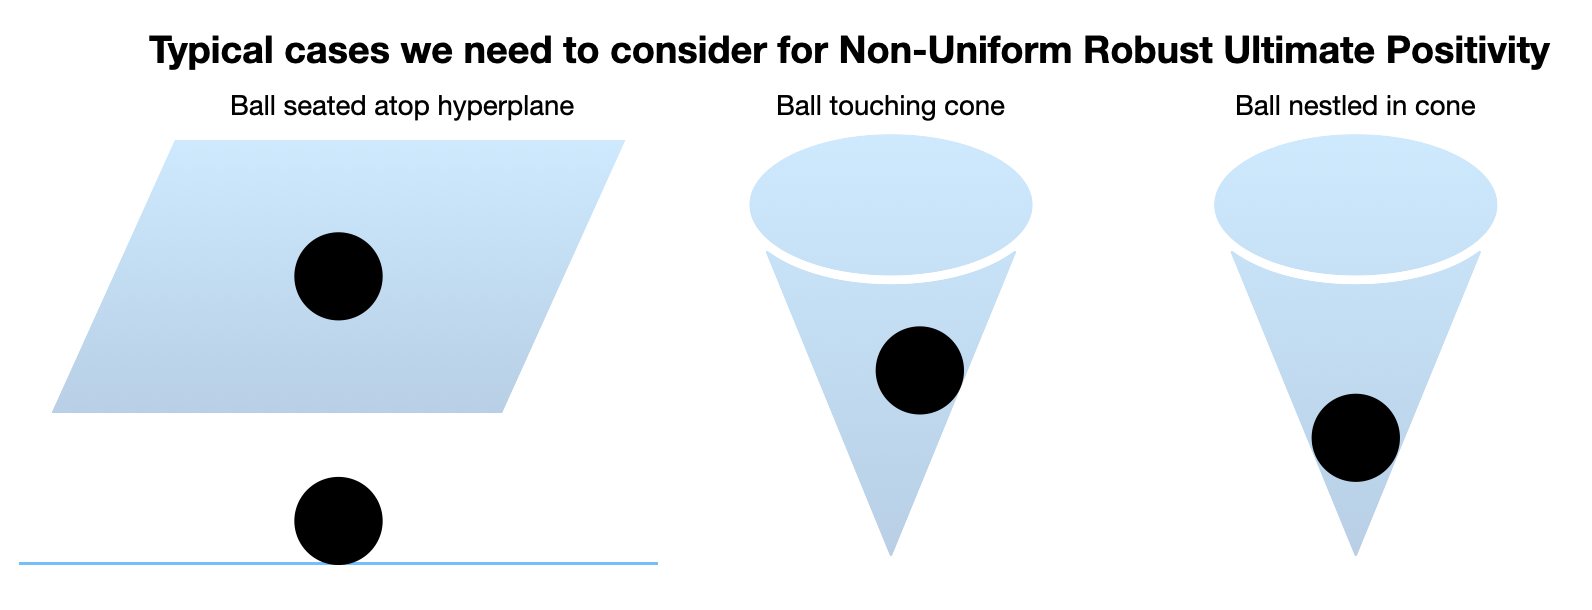
\includegraphics[width=\textwidth]{picture1.png}
\caption{Visual intuition. The region $\mu \ge 0$ is defined by the intersection of halfspaces. The orientation of the neighbourhood relative to this region is deduced with the First Order Theory of the Reals. When there are finitely many halfspaces, the critical case is marked by the ball being tangent to the separating hyperplane(s) at finitely many discrete points. In low dimensions, Ultimate Positivity can be decided for these boundary cases using existing techniques. When there are infinitely many halfspaces, they carve out a region that resembles a cone. The neighbourhood can either touch the cone as before, or be nestled in it, having a continuous, connected region of tangency. In the latter case, Robust Ultimate Positivity can be handled with number-theoretic arguments in the low-dimensional setting.}
\label{fig:geometricpicture}
\end{figure}

We adopt this strategy (see Figure \ref{fig:geometricpicture}) and prove our second decidability result in \S\ref{section:decidability2}.
\begin{theorem}[Second Decidability Result]
\label{thm:decide2}
Problem \ref{prob:rrobnonuniultpos} is decidable up to order 4.
\end{theorem}




